\documentclass[a4paper,12pt]{article}

\usepackage[utf8]{inputenc}
\usepackage{lmodern}
\usepackage[margin=1cm]{geometry}
\usepackage{amsmath}
\usepackage{graphicx}
\usepackage{xcolor}
\usepackage{caption}
\usepackage{tikz}
\usetikzlibrary{arrows.meta,positioning,shapes.geometric,calc,fit}

\pagestyle{empty}

\begin{document}
\begin{figure}[p]
  \centering
  \vspace*{-1.0cm}
  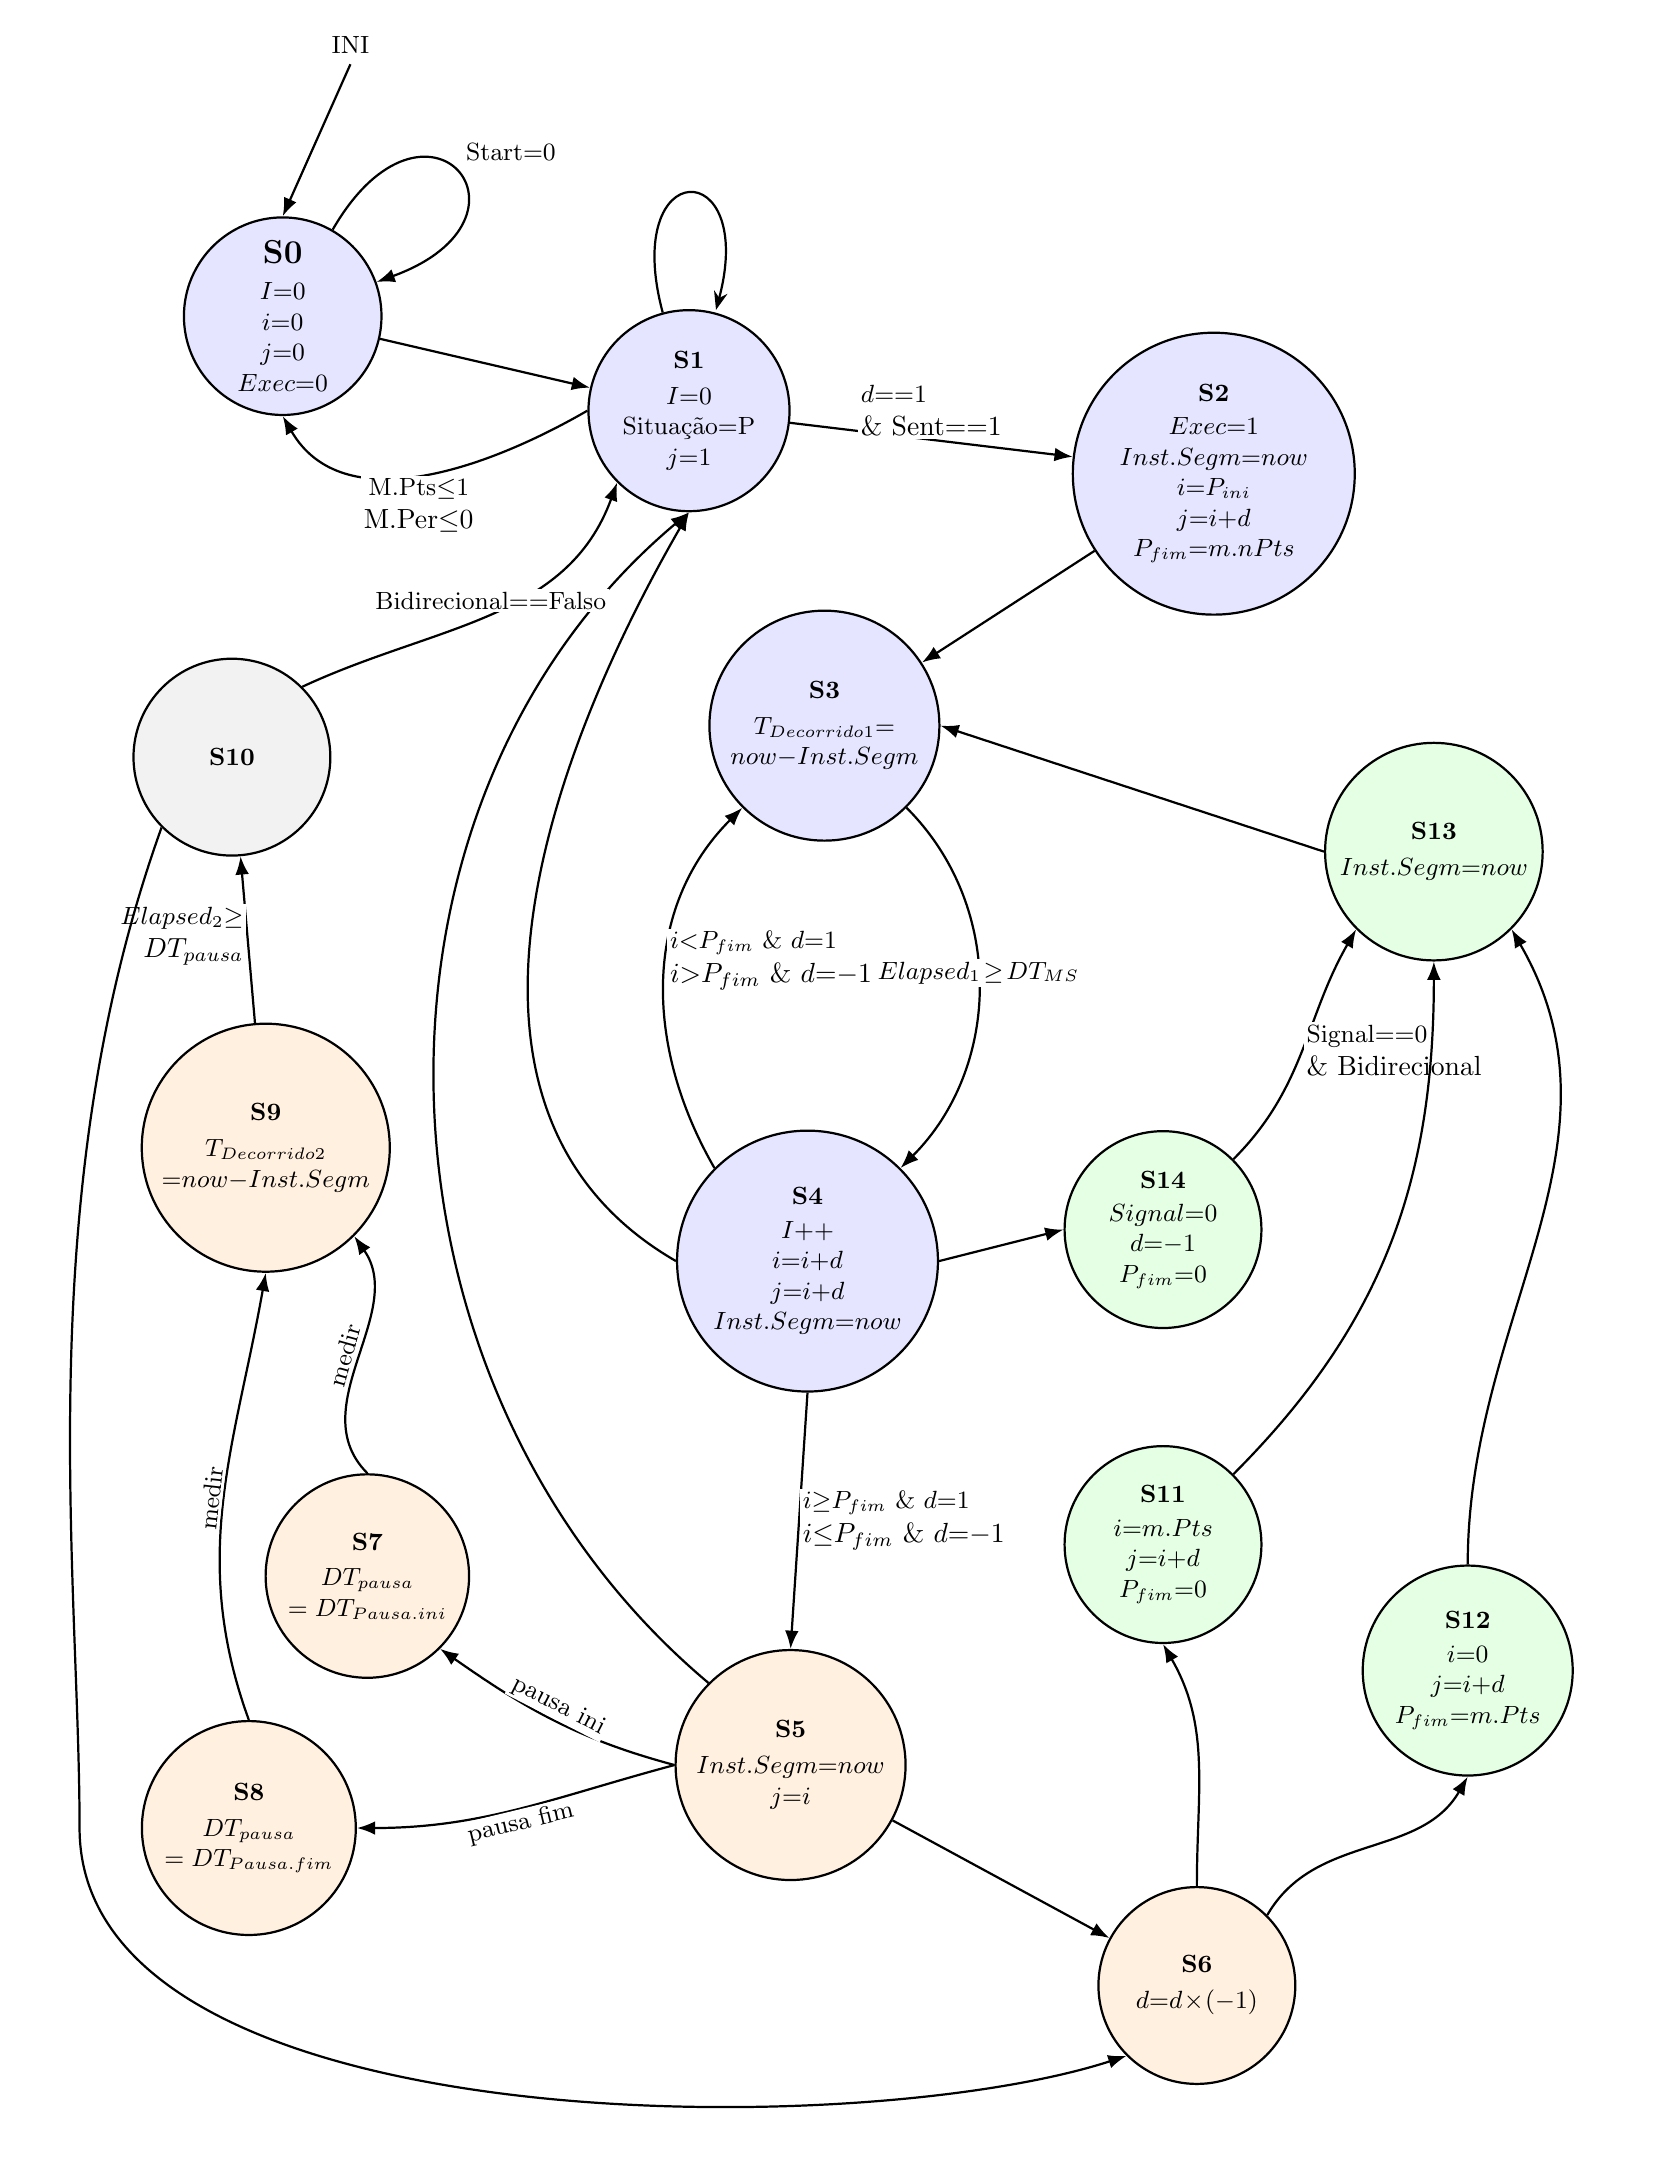
\begin{tikzpicture}[
    x=0.43cm,
    y=0.80cm,
    state/.style={draw, circle, align=center, minimum size=2.5cm, font=\small, thick, inner sep=3pt},
    arrow/.style={-Latex, thick},
    rlabel/.style={fill=white, inner sep=1pt},
    >=Stealth
  ]
    % ── Nome do estado a negrito no topo, variáveis abaixo ──
    \node[state, fill=blue!10]   (s0)  at (-12.0, 28) {{\large\textbf{S0}}\\[2pt]$I{=}0$\\$i{=}0$\\$j{=}0$\\$Exec{=}0$};
    \node[state, fill=blue!10]   (s1)  at (0.0, 26.5) {\textbf{S1}\\[2pt]$I{=}0$\\Situa\c{c}\~ao$=$P\\$j{=}1$};
    \node[state, fill=blue!10] (s2) at (15.5, 25.5) {\textbf{S2}\\[1pt]$Exec{=}1$\\$Inst.Segm{=}now$\\$i{=}P_{ini}$\\$j{=}i{+}d$\\$P_{fim}{=}m.nPts$};
    \node[state, fill=blue!10]   (s3)  at (4.0, 21.5) {\textbf{S3}\\[2pt]$T_{Decorrido1}{=}$\\$now{-}Inst.Segm$};
    \node[state, fill=blue!10] (s4) at (3.5, 13.0) {\textbf{S4}\\[1pt]$I{+}{+}$\\$i{=}i{+}d$\\$j{=}i{+}d$\\$Inst.Segm{=}now$};
    \node[state, fill=green!10]  (s13) at (22.0, 19.5) {\textbf{S13}\\[2pt]$Inst.Segm{=}now$};
    \node[state, fill=green!10]  (s14) at (14.0, 13.5)  {\textbf{S14}\\[1pt]$Signal{=}0$\\$d{=}{-}1$\\$P_{fim}{=}0$};
    \node[state, fill=green!10] (s11) at (14.0, 8.5) {\textbf{S11}\\[1pt]$i{=}m.Pts$\\$j{=}i{+}d$\\$P_{fim}{=}0$};
    \node[state, fill=green!10] (s12) at (23.0, 6.5) {\textbf{S12}\\[1pt]$i{=}0$\\$j{=}i{+}d$\\$P_{fim}{=}m.Pts$};
    \node[state, fill=orange!12] (s5)  at (3.0, 5.0) {\textbf{S5}\\[2pt]$Inst.Segm{=}now$\\$j{=}i$};
    \node[state, fill=orange!12] (s6)  at (15.0, 1.5)  {\textbf{S6}\\[2pt]$d{=}d\!\times\!({-}1)$};
    \node[state, fill=orange!12] (s7)  at (-9.5, 8.0) {\textbf{S7}\\[2pt]$DT_{pausa}$\\$=DT_{Pausa.ini}$};
    \node[state, fill=orange!12] (s8)  at (-13.0, 4.0)  {\textbf{S8}\\[2pt]$DT_{pausa}$\\$=DT_{Pausa.fim}$};
    \node[state, fill=orange!12] (s9)  at (-12.5, 14.8) {\textbf{S9}\\[2pt]$T_{Decorrido2}$\\${=}now{-}Inst.Segm$};
    \node[state, fill=gray!10]   (s10) at (-13.5, 21.0) {\textbf{S10}};

    % ── Seta de início ──
    \draw[arrow] (-10, 32.0) node[above]{\small INI} -- (s0.north);

    % ── S0: loop e saída ──
    \draw[arrow] (s0) edge[loop, out=60, in=20, looseness=7] node[above right]{\small Start$=$0} (s0);
    \draw[arrow] (s0) -- (s1);

    % ── S1: loop e retorno a S0 ──
    \draw[arrow] (s1) edge[loop above] node[above]{} (s1);
    \draw[arrow] (s1.west) to[out=-150, in=-60] node[rlabel, below, align=center]{\small M.Pts$\le$1\\M.Per$\le$0} (s0.south);

    % ── S1 → S2 ──
    \draw[arrow] (s1) -- node[rlabel, above, align=left]{\small $d{==}1$\\\& Sent$==$1} (s2);

    % ── Cadeia principal S2→S3→S4 ──
    \draw[arrow] (s2) -- (s3);
    \draw[arrow] (s3.south east) to[out=-45, in=45] node[rlabel, pos=0.50, above, align=center]{\small $Elapsed_1\!\ge\!DT_{MS}$} (s4.north east);

    % ── S4: retorno a S3 ──
    \draw[arrow] (s4.north west) to[out=120, in=-135] node[rlabel, pos=0.55, right, align=left]{\small $i{<}P_{fim}$ \& $d{=}1$\\$i{>}P_{fim}$ \& $d{=}{-}1$} (s3.south west);

    % ── S4 → S5 ──
    \draw[arrow] (s4.south) -- node[rlabel, right, align=left]{\small $i{\ge}P_{fim}$ \& $d{=}1$\\$i{\le}P_{fim}$ \& $d{=}{-}1$} (s5.north);

    % ── S4 → S14 ──
    \draw[arrow] (s4.east) -- (s14.west);

    % ── S4 → S1 ──
    \draw[arrow] (s4.west) to[out=150, in=-120] (s1.south);

    % ── S5 → S1 ──
    \draw[arrow] (s5.north west) to[out=140, in=-140] (s1.south);

    % ── S13 → S3 ──
    \draw[arrow] (s13.west) -- (s3.east);

    % ── S14 → S13 ──
    \draw[arrow] (s14.north east) to[out=45, in=-120] node[rlabel, right, align=left]{\small Signal$==$0\\\& Bidirecional} (s13.south west);

    % ── S11 → S13 / S12 → S13 ──
    \draw[arrow] (s11.north east) to[out=45, in=-90] (s13.south);
    \draw[arrow] (s12.north) to[out=90, in=-60] (s13.south east);

    % ── S5 → S6 ──
    \draw[arrow] (s5) -- (s6);

    % ── S6 → S11 / S6 → S12 ──
    \draw[arrow] (s6.north) to[out=90, in=-60] (s11.south);
    \draw[arrow] (s6.north east) to[out=60, in=-120] (s12.south);

    % ── S5 para pausas ──
    \draw[arrow] (s5.west) to[out=165, in=-35] node[rlabel, pos=0.50, above, sloped]{\small pausa ini} (s7.south east);
    \draw[arrow] (s5.west) to[out=195, in=0] node[rlabel, pos=0.50, below, sloped]{\small pausa fim} (s8.east);

    % ── S7 → S9 ──
    \draw[arrow] (s7.north) to[out=135, in=-55] node[rlabel, pos=0.50, above, sloped]{\small medir} (s9.south east);

    % ── S8 → S9 ──
    \draw[arrow] (s8.north) to[out=110, in=-100] node[rlabel, pos=0.50, above, sloped]{\small medir} (s9.south);

    % ── S9 → S10 ──
    \draw[arrow] (s9) -- node[rlabel, pos=0.52, left, align=right]{\small $Elapsed_2{\ge}$\\$DT_{pausa}$} (s10);

    % ── S10 → S1 ──
    \draw[arrow] (s10.north east) to[out=25, in=-110] node[rlabel, pos=0.50, above]{\small Bidirecional$==$Falso} (s1.south west);
    \draw[arrow] (s10.south west)
        .. controls (-19.5, 14) and (-18, 8) .. (-18, 4)
        .. controls (-18, -1) and (5, -1) .. (s6.south west);
  \end{tikzpicture}
  \caption{Esquema da FSM\_Motion\_Update.}
  \label{fig:fsm-motion}
\end{figure}

\end{document}
